\begin{frame}{Conclusiones a nivel de proyecto}
  \begin{block}{Objetivos cumplidos}
    Se completaron todos los objetivos propuestos:
    \begin{itemize}
    \item Se creó un módulo de análisis de notas eficiente.
    \item El sistema de canciones integró el módulo de análisis de forma
      efectiva.
    \item Desarrollamos un sistema de lecciones muy completo.
    \item Se mantuvo en todo momento una interfaz agradable y fluida.
    \end{itemize}    
  \end{block} 
\end{frame}

\begin{frame}{Conclusiones a nivel de proyecto}
  \begin{block}{Posibles mejoras}
    Hay lugar para ampliar el proyecto:
    \begin{itemize}
    \item Extender el sistema de lecciones para añadir, por ejemplo, vídeos y
      otros elementos multimedia.
    \item Mejorar la jugabilidad del sistema de canciones.
    \item Portar el juego a otras plataformas.
    \end{itemize}
  \end{block}  
\end{frame}

\begin{frame}{Conclusiones a nivel personal}
  \begin{itemize}
  \item Proyecto muy longevo.
  \item Mucho conocimiento nuevo adquirido: DSP, programación de audio, hilos,
    matemáticas...
  \item Mucho conocimiento generado.
  \item Cercano a proyectos comerciales.
  \end{itemize}
\end{frame}

\begin{frame}{Conocimiento generado}
  \pause

  \begin{block}{Taller de Boost}
    Se explicaron las partes más importantes de esta colección de bibliotecas,
    con numerosos ejemplos.
  \end{block}

  \pause

  \begin{block}{Taller de Gosu}
    Más de 50 asistentes, desarrollo de un clon del Arkanoid.
  \end{block}

  \pause

  \begin{block}{Tutorial de Gettext}
    Completo manual de internacionalización de proyectos. También se hizo un
    taller sobre el mismo tema.
  \end{block}
\end{frame}

\begin{frame}{Proyectos derivados}

  \begin{center}
    A partir del código de oFlute se desarrolló \textbf{Freegemas}, clon
    libre y multiplataforma de Bejeweled.

    \medskip

    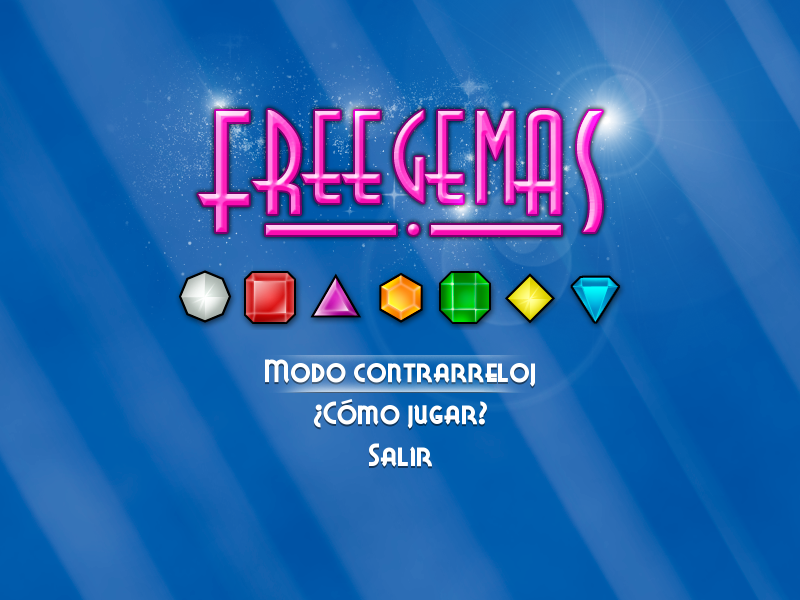
\includegraphics[width=0.49\textwidth]{imagenes/imagen_freegemas1}\hspace{0.1cm}
    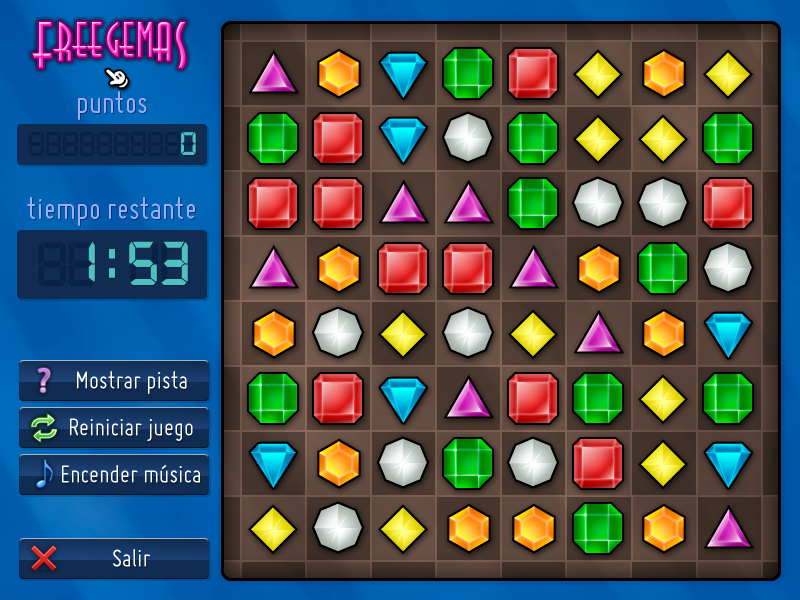
\includegraphics[width=0.49\textwidth]{imagenes/imagen_freegemas2}

    \medskip

    \begin{itemize}
    \item \textbf{Tres publicaciones} en Linux Magazine.
    \item \textbf{Inclusión oficial} en Guadalinex v8.
    \end{itemize}
  \end{center}
\end{frame}

\begin{frame}{Difusión}
  \begin{block}{Social media}
    \begin{itemize}
    \item Blog: \url{oflute.wordpress.com}, 5500 visitas en total.
    \item 3 vídeos en YouTube, aprox. 700 reproducciones.
    \end{itemize}    
  \end{block}

  \pause

  \begin{block}{Forja}
    \begin{itemize}
    \item \url{http://oflute.googlecode.com}
    \item Más de 270 revisiones.
    \item Aprox. 8000 líneas de código.
    \end{itemize}
  \end{block}

  \pause

  \begin{block}{Referencia del código}
    \begin{itemize}
    \item Generada con \textbf{Doxygen}.
    \item Disponible en la forja.
    \item Accesible en \url{http://www.josetomastocino.com/oflute}.
    \end{itemize}
  \end{block}
\end{frame}

\begin{frame}{Difusión}
  \begin{block}{Concurso Universitario de Software Libre}
    \begin{itemize}
    \item Mención especial a nivel nacional.
    \item Accésit al mejor proyecto de innovación en la fase local.
    \end{itemize}
  \end{block}
  
  \pause

  \begin{block}{Guadalinex}
    \begin{itemize}
    \item oFlute se encuentra  en los repositorios de \textbf{Guadalinex}.
    \end{itemize}
  \end{block}
\end{frame}
%%% Local Variables: 
%%% mode: latex
%%% TeX-master: "../presentacion"
%%% End: 
